\section*{Appendix}
\addcontentsline{toc}{section}{Appendix}

\noindent {\bf Data and Code Availability}

\noindent For the purposes of transparency and reproducibility, all data and source code utilized in this study are publicly accessible in the following \href{https://github.com/yildirimalper/yildirim-masters-thesis}{GitHub repository}. \\

%\noindent {\bf Estimation of Yield Curve with Nelson-Siegel-Svensson Model}

%\noindent In their seminal paper, \citet{nelson1987parsimonious} specifies the forward rate curve $\tau(f)$ as follows:

%\begin{equation}\notag
%    f(\tau)=
%    \begin{pmatrix}
%    \beta_0 \\ \beta_1 \\ \beta_2    
%    \end{pmatrix}'
%     \begin{pmatrix}
%         1 \\ e^{-\tau/\lambda} \\ (\tau / \lambda) e^{-\tau/\lambda}
%     \end{pmatrix}
%     =
%     \begin{pmatrix}
%     \beta_0 \\ \beta_1 \\ \beta_2   
%     \end{pmatrix}'
%     \begin{pmatrix}
%     f_0 \\ f_1 \\ f_2  
%     \end{pmatrix}
% \end{equation}


% Ridge reg paper'ından aynen aldım
% \noindent The spot rate function, which is the average of the forward rate curve up to time to maturity $\tau$, is defined as:

% \begin{equation}\notag
%    r(\tau)= \frac{1}{\tau}\int_0^\tau f(u)\,du
% \end{equation}

% \noindent with continuous compounding. Hence, the corresponding spot rate function at time to maturity $\tau$ reads


\noindent {\bf Estimation of Corwin-Schultz Bid-Ask Spread}

\noindent \citet{corwin2012simple} constructed a bid-ask spread estimator using the daily high and low prices. The estimator is based on this insight: During trading, when prices fluctuate, the highest price is likely due to a buyer actively pushing the price up, crossing the spread, and matching the ask. Conversely, the lowest price likely results from a seller pushing the price down, crossing the spread, and matching the bid. Let $H$ and $L$ denote intraday highest and lowest price, respectively. That is, the two-day high and low observations are:
$$
H_{t,t+1} = \max(H_t, H_{t+1})\quad\quad L_{t,t+1} = \max(L_t, L_{t+1})
$$

\noindent The sample estimates for the Corwin-Schultz model are:
$$
\begin{aligned}
\hat{\gamma}&=\left[\ln \left(\frac{H_{t, t+1}}{L_{t, t+1}}\right)\right]^2 \\
\hat{\beta}&=\left(\ln \left(\frac{H_t}{L_t}\right)+\ln \left(\frac{H_{t+1}}{L_{t+1}}\right)\right)^2
\end{aligned}
$$

\noindent Under certain assumptions, the closed form for expression become:

$$
\alpha=\frac{\sqrt{2 \beta}-\sqrt{\beta}}{3-2 \sqrt{2}}-\sqrt{\frac{\gamma}{3-2 \sqrt{2}}}
$$

$$
\hat{S}_{H L}=\frac{2\left(e^\alpha-1\right)}{1+e^\alpha}
$$

\newpage

\noindent The corresponding Python code used in this study:
\begin{mintedbox}{python}
def HLSpreadEstimator(highs, lows):
    beta = (np.log(highs[0] / lows[0]))**2 + (np.log(highs[1] / lows[1]))**2
    H = max(highs)
    L = min(lows)
    gamma = (np.log(H / L))**2
    alpha = (np.sqrt(2 * beta) - np.sqrt(beta)) / (3 - 2 * np.sqrt(2)) - np.sqrt(gamma / (3 - 2 * np.sqrt(2)))
    s = (2 * (np.exp(alpha) - 1)) / (1 + np.exp(alpha))
    s = max(s, 0)
    return s
\end{mintedbox}

\vspace{1.5cm}

\noindent { \bf Historical Interest Rates}

\begin{figure}[H]
    \centering
    \caption{Long-Term Nominal Interest Rates}
    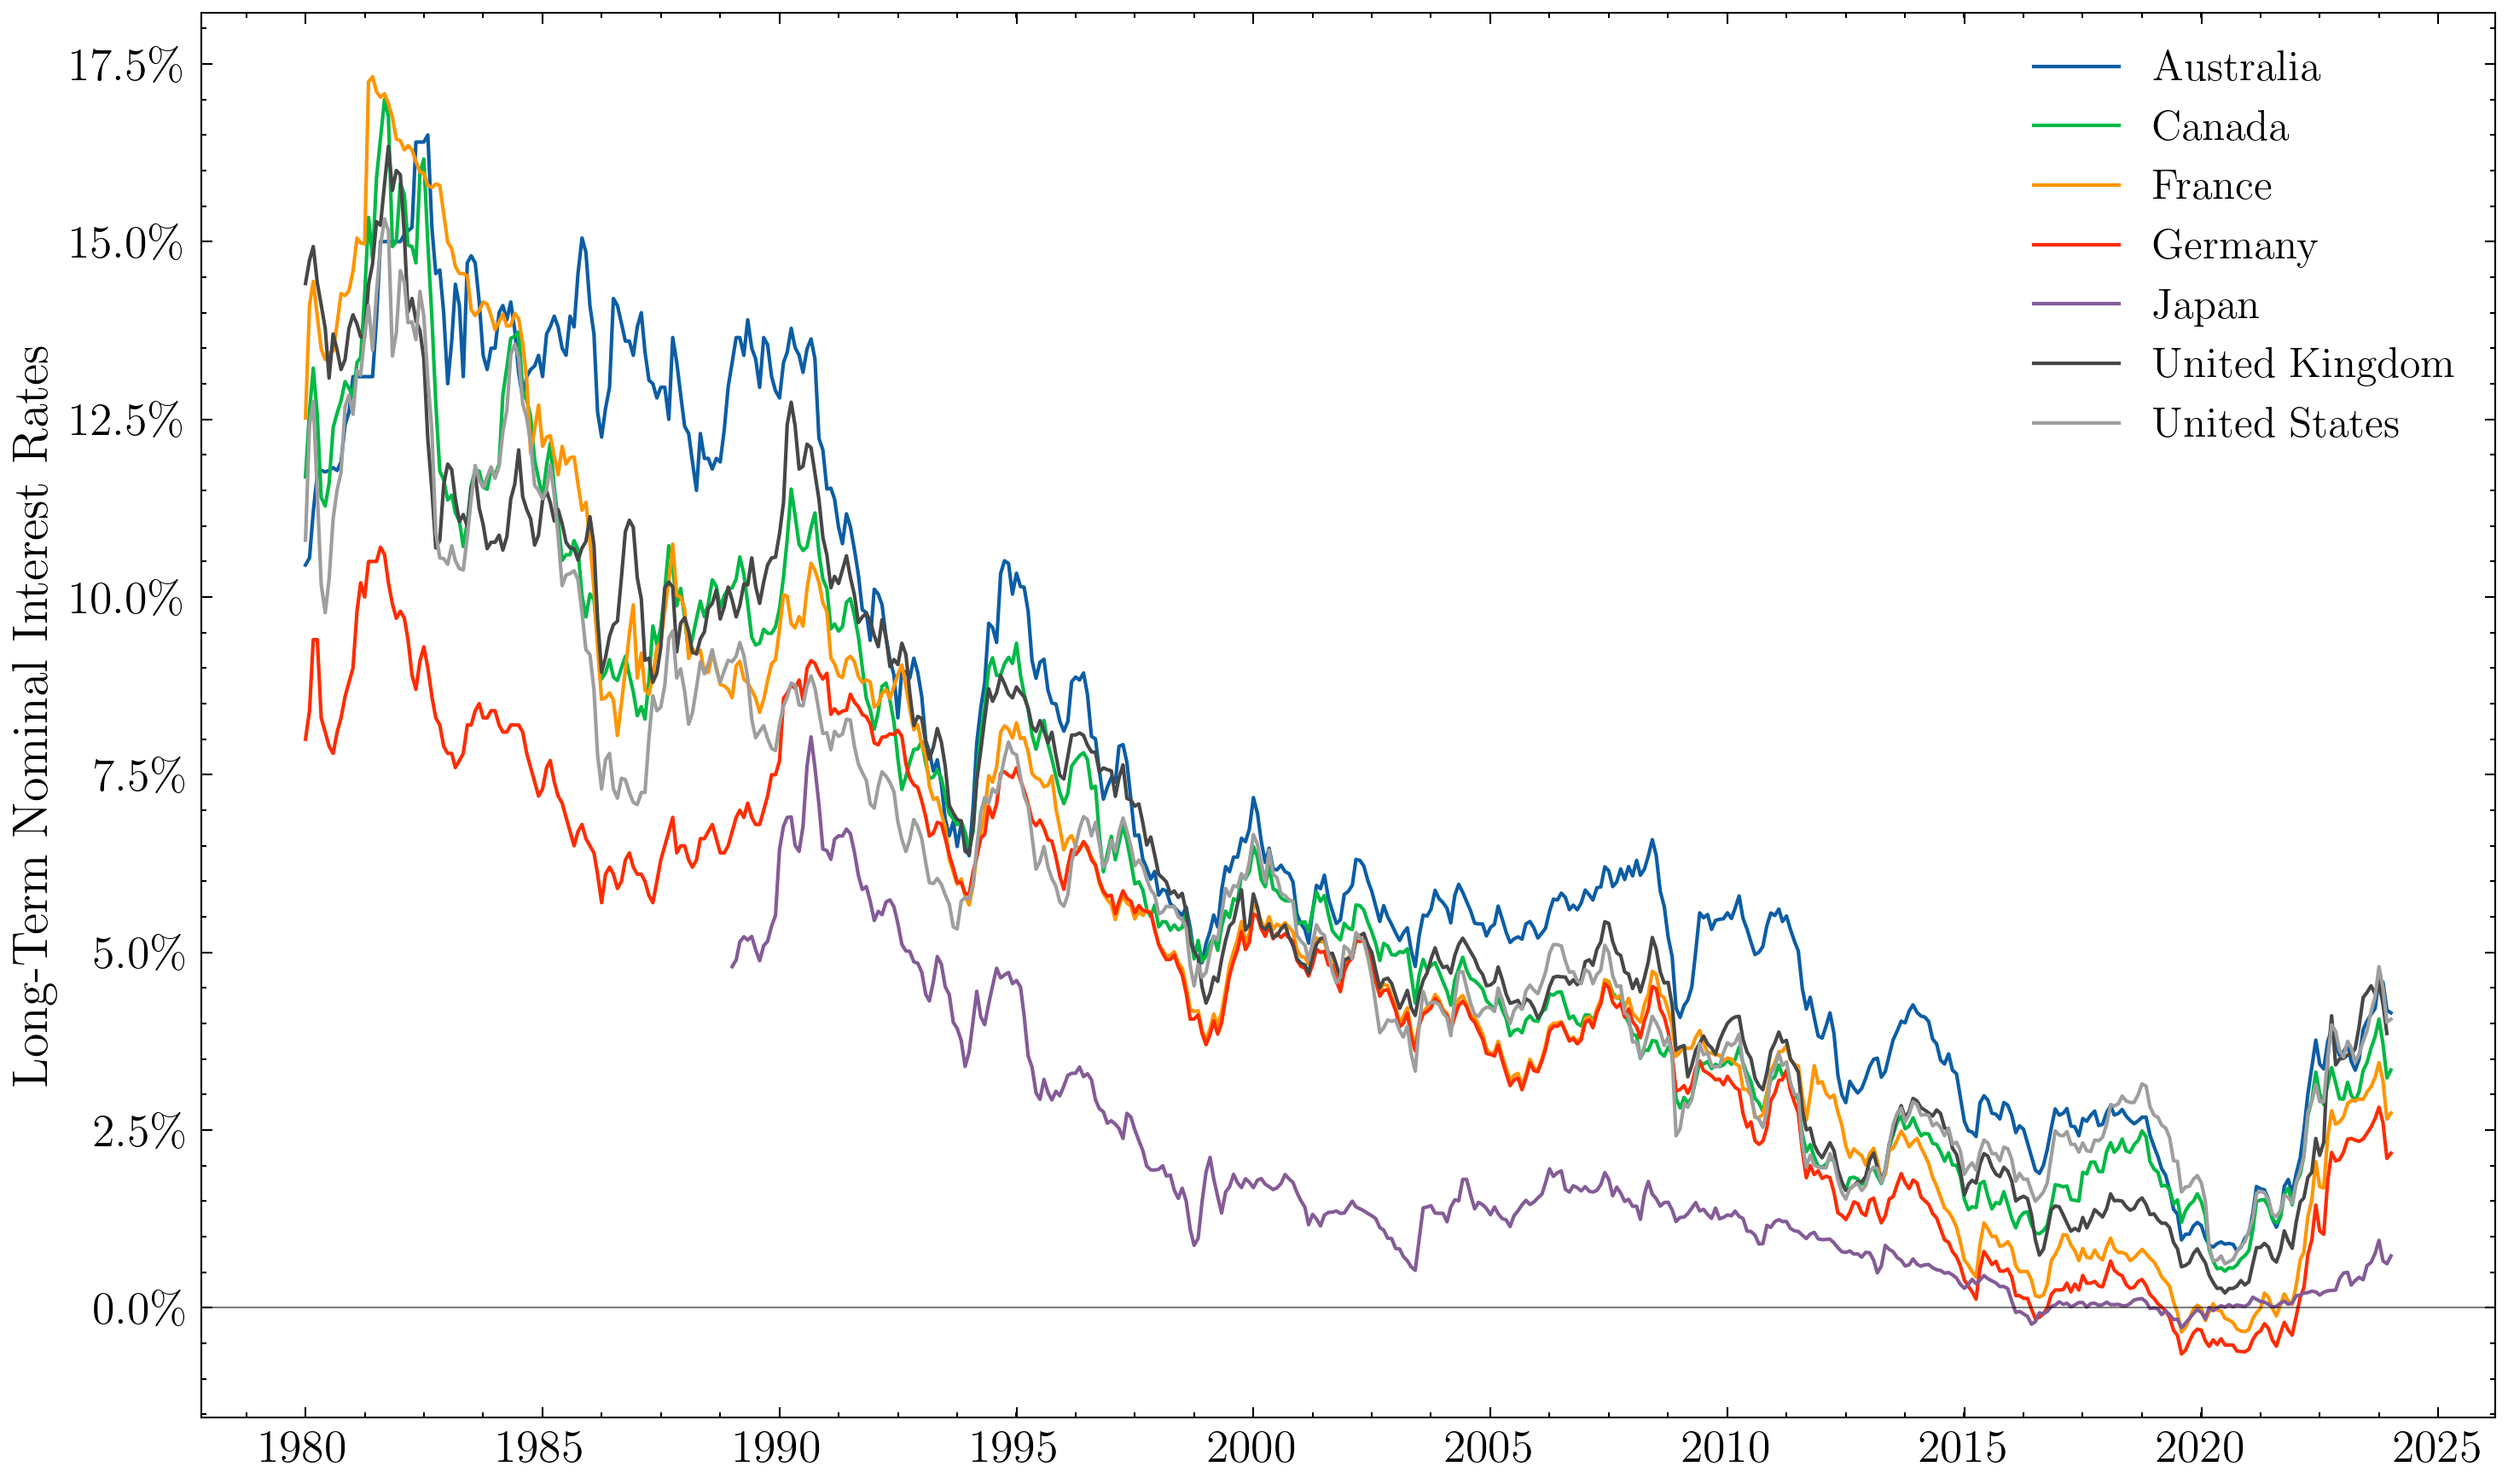
\includegraphics[width=0.8\textwidth]{figures/long-term-rates.png}
    
    \vspace{15pt}
    
    \begin{minipage}{\textwidth}
        \footnotesize % Adjust font size to 8pt
        \textbf{Note:} In this figure, long-term interest rates refer to 10-year bond yields. The data is obtained from OECD Database.
    \end{minipage}
    \label{fig:long-term-rates}
\end{figure}

\newpage

\begin{table}[htbp!]
    \centering
    \caption{Historical Credit Ratings of Sampled Countries}
    \renewcommand\arraystretch{0.9}
    \small
    \begin{tabular}{L{3.5cm}C{3.5cm}C{3.5cm}C{3.5cm}}
        \toprule
        \rowcolor[HTML]{C0C0C0} % Light grey color for the header
        & \textbf{S\&P} & \textbf{Moody's Ratings} & \textbf{Fitch Ratings} \\
        \midrule
        \rowcolor[HTML]{EFEFEF} 
        \textbf{Germany} & & & \\
        \midrule
        2024 & AAA & Aaa & AAA \\
        1994 &  &  & AAA \\
        1986 & & Aaa & \\
        1983 & AAA & & \\
        \midrule
        \rowcolor[HTML]{EFEFEF} 
        \textbf{United Kingdom} & & & \\
        \midrule
        2024 & AA & Aa3 & AA- \\
        2020 & & Aa3 & AA- \\
        2017 & & Aa2 & \\
        2016 & AA & & AA \\
        2013 & & Aa1 & AA+ \\
        1994 & & & AAA  \\
        1978 & AAA & Aaa & \\
        \midrule
        \rowcolor[HTML]{EFEFEF} 
        \textbf{Japan} & & & \\
        \midrule
        2024 & A+ & A1 & A \\
        2015 & A+ & & A \\
        2014 & & A1 & \\
        2012 & & &  \\
        2011 & AA- & Aa3 & \\
        2009 & & Aa2 & \\
        2007 & AA & & \\
        2004 & & Aaa & \\
        2002 & AA- & & \\
        2001 & AA & & AA \\
        2000 & & & AA+\\
        1998 & & Aa1 & \\
        1994 & & & AAA \\
        1981 & & Aaa & \\
        1975 & AAA & & \\
        \bottomrule
    \end{tabular}
\end{table}

\newpage


\begin{table}[htbp!]
    \centering
    \renewcommand\arraystretch{0.9}
    \small
    \begin{tabular}{L{3.5cm}C{3.5cm}C{3.5cm}C{3.5cm}}

        \toprule
        \rowcolor[HTML]{C0C0C0}
        & \textbf{S\&P} & \textbf{Moody's Ratings} & \textbf{Fitch Ratings} \\
        \midrule
        \rowcolor[HTML]{EFEFEF}
        \textbf{Canada} & & & \\
        \midrule
        2024 & AAA & Aaa & AA+ \\
        2020 & & & AA+ \\
        2004 & & & AAA \\
        2002 & AAA & Aaa & \\
        2001 & & & AA+ \\
        2000 & & Aa1 & \\
        1995 & & Aa2 & \\
        1994 & & Aa1 & AA \\
        1992 & AA+ & & \\
        1974 & & Aaa & \\
        \midrule
        \rowcolor[HTML]{EFEFEF} 
        \textbf{Switzerland} & & & \\
        \midrule
        2024 & AAA & Aaa & AAA \\
        2000 & & & AAA \\
        1999 & & & AA \\
        1994 & & & AA- \\
        1994 & & & AA \\
        1988 & AAA & & \\
        1982 & & Aaa & \\
        \midrule
        \rowcolor[HTML]{EFEFEF}
        \textbf{Australia} & & & \\
        \midrule
        2024 & AAA & Aaa & AAA \\
        2011 & & & AAA \\
        2003 & AAA & & AA+ \\
        2002 & & Aaa & \\
        1999 & AA+ & & \\
        1996 & & & AA \\
        1989 & AA & Aa2 & \\
        1986 & AA+ & Aa1 & \\
        % Add more years and ratings as needed
        \bottomrule
    \end{tabular}
\end{table}
\\

{\footnotesize \noindent \textbf{Note:} The data is obtained from the \href{https://www.worldgovernmentbonds.com/world-credit-ratings/}{World Government Bonds}}.
